\chapter{Badania eksperymentalne}

\section{Opis eksperymentów}
\section{Zaimplementowane algorytmy}
\subsection{Próbkowanie dwufazowe}
Próbkowanie dwufazowe swoją nazwę zawdzięcza procesowi próbkowania składającemu się z dwóch oddzielnych faz
- próbkowania wierzchołków oraz próbkowania krawędzi - wykonywanych jedna po drugiej.
Istotną zaletą tego podejścia jest jego stosunkowo prosta implementacja.

Zaimplementowany algorytm pochodzi z pracy\cite{DBLP:conf/depcos/BozejkoGNAB18}.
Został on przygotowany specjalnie do próbkowania przestrzeni rozwiązań problemu komiwojażera.
Próbkowanie wierzchołków odbywa się poprzez generowanie losowych rozwiązań, a następnie ich optymalizacji algorytmem 2-opt.
Próbkowanie krawędzi polega na wielokrotnym poddaniu każdego ze znalezionych wcześniej lokalnych optimów $n_i$ operacji perturbacji typu 2-exchange,
a następnie poddaniu powstałego rozwiązania optymalizacji algorytmem 2-opt typu \textit{first-improvement} uzyskując w ten sposób lokalne optimum $n_j$.
Następnie dodawana jest krawędź między $n_i$ a $n_j$, lub - jeśli już taka istnieje - jej waga jest zwiększana o 1.

Algorytm przyjmuje trzy parametry: pożądaną liczbę wierzchołków do wygenerowania ($n_{max}$), maksymalną liczbę prób generowania wierzchołka ($n_{att}$)
oraz maksymalną liczbę prób generowania krawędzi($e_{att}$).
Implementacja zastosowana w tej pracy dodatkowo powtarza cały proces kilkukrotnie, za każdym razem zapisując zebrane próbki do pliku.

Algorytm w postaci pseudokodu został przedstawiony na listingu \ref{alg:tp}.

\subsection{Snowball}
Próbkowanie typu Snowball wywodzi się z techniki używanej w badaniach z dziedziny socjologii, w której ludzie należący do próby z populacji
rekrutują kolejnych uczestników badania spośród swoich znajomych.
W kontekście badania przestrzeni rozwiązań technika ta została zaprezentowana w pracy\cite{DBLP:conf/ppsn/VerelDOT18}, gdzie została wykorzystana
do próbkowanie przestrzeni problemu kwadratowego przypisania (QAP).

Próbkowanie składa się z etapów procedury \textit{snowball} próbkującej "wgłąb" i losowego spaceru(ang. \textit{random walk}).
Próbkowanie \textit{snowball} polega na wybraniu rozwiązania startowego i przeszukaniu jego najbliższego sąsiedztwa.
Następnie operacja ta jest powtarzana dla każdego rozwiązania w tym sąsiedztwie. Proces powtarza się aż do osiągnięcia z góry ustalonej głebokości
przeszukiwania. Następnie rozpoczyna się procedura losowego spaceru - wybierane jest kolejne rozwiązanie startowe
ze zbioru sąsiadów poprzedniego rozwiązywania startowego (lub rozwiązanie losowe, jeśli to sąsiedztwo jest puste) i proces \textit{snowball}
rozpoczyna się od nowa. Procedura jest powtarzana aż osiągnięty zostanie z góry ustalony limit długości spaceru.

Zaimplementowany algorytm jest próbą adaptacji tej techniki do zadania przeszukiwania przestrzeni
problemu komiwojażera. Do najważniejszych modyfikacji należy zastąpienie funkcji optymalizacji lokalnej \textit{hillclimb}
optymalizacją 2opt, implementacja odpowiedniej funkcji celu oraz operacji mutacji typu 2-exchange.

Algorytm w postaci pseudokodu został przedstawiony na listingu \ref{alg:snowball}.

\begin{algorithm}[h!]
    \caption{Próbkowanie dwufazowe - pseudokod}\label{alg:tp}

    \KwData{\\
        \Indp \Indp
        $n_{max}$ - żądana liczba wierzchołków\\
        $n_{att}$ - liczba prób generowania wierzchołków\\
        $e_{att}$ - liczba prób generowania krawędzi\\
        $n_{runs}$ - liczba powtórzeń\\
        $D$ - stała D krawędzi
    }

    \vspace{1em}

    $N \gets \{\}$\;
    $E \gets \{\}$\;
    \For{$i\gets1$ \KwTo $n_{runs}$}{
        $probkujWierzcholki(N, n_{max}, n_{att})$\;
        $probkujKrawedzie(N, E, e_{att})$\;
        $zapiszDoPliku(N, E)$\;
    }
    \vspace{1em}

    \SetKwFunction{FV}{probkujWierzcholki}
    \SetKwProg{Fn}{function}{:}{}

    \Fn{\FV{$N, n_{max}, n_{att}$}}{
        \For{$i\gets1$ \KwTo $n_{max}$}{
            \For{$i\gets1$ \KwTo $n_{att}$}{
                $s \gets losoweRozwiazanie()$\;
                $s \gets 2opt(s)$\;
                $N \gets N \cup \{s\}$\;
            }
        }
    }
    \textbf{end}

    \vspace{1em}

    \SetKwFunction{FE}{probkujKrawedzie}

    \Fn{\FE{$N, E, e_{att}$}}{
        \ForEach{$n \in{N}$}{
            \For{$i\gets1$ \KwTo $e_{att}$}{
                $s \gets 2exchangeMutacja(n, D)$\;
                $s \gets 2optFirstImprovement(s)$\;
                \If{$s \in{N}$}{
                    $E \gets E \cup \{(n, s)\}$\;
                    $w_{ns} \gets w_{ns} + 1$\;
                }
            }
        }
    }
    \textbf{end}

    \vspace{1em}

\end{algorithm}

\newpage

\begin{algorithm}[h!]
    \caption{Próbkowanie snowball - pseudokod}\label{alg:snowball}

    \KwData{\\
        \Indp \Indp
        $w_{len}$ - długość losowego spaceru\\
        $m$ - liczba prób przeszukania sąsiedztwa\\
        $depth$ - głębokość przeszukiwania\\
        $n_{runs}$ - liczba powtórzeń\\
        $D$ - stała D krawędzi
    }

    \vspace{1em}
    $s_1 \gets losoweRozwiazanie()$\;
    $n_1 \gets 2opt(s_1)$\;

    $N \gets \{ n_1 \}$\;
    $E \gets \{\}$\;
    \For{$j\gets1$ \KwTo $n_{runs}$}{
        \For{$i\gets1$ \KwTo $w_{len}$}{
            $snowball(n_i, m, depth)$\;
            $n_{i+1} \gets losowySpacer(n_i)$\;
        }
        $zapiszDoPliku(N, E)$\;
    }
    \vspace{1em}

    \SetKwFunction{FS}{snowball}
    \SetKwProg{Fn}{function}{:}{}

    \Fn{\FS{$n, m, depth$}}{
        \If{$d > 0$}{
            \For{$i\gets1$ \KwTo $m$}{
                $s \gets 2opt(2exchangeMutacja(n, D))$\;
                $N \gets N \cup \{ s \}$\;
                \uIf{$(n, s) \in{E}$}{
                    $w_{ns} \gets w_{ns} + 1$\;
                }
                \Else{
                    $E \gets E \cup \{ (n, s) \}$\;
                    $w_{ns} \gets 1$\;
                    $snowball(s, m, d-1)$\;
                }
            }
        }
    }
    \textbf{end}

    \vspace{1em}

    \SetKwFunction{FW}{losowySpacer}

    \Fn{\FW{$n_i$}}{
        $neighbours \gets \{ s: (n_i, s) \in E \land s \notin \{ n_0...n_i \} \}$\;
        \uIf{$neighbours \neq \emptyset $}{
            $n_{i+1} \gets losowyElementZeZbioru(neighbours)$\;
        }
        \Else{
            $s \gets losoweRozwiazanie()$\;
            $n_{i+1} \gets 2opt(s)$\;
            $N \gets N \cup \{ n_{i+1} \}$\;
        }
        \Return $n_{i+1}$
    }
    \textbf{end}

    \vspace{1em}

\end{algorithm}

\newpage

\subsection{Przegląd zupełny}
Ze względu na złożoność problemu komiwojażera przegląd zupełny można zastosować tylko do bardzo małych instancji problemu.
Przegląd polega na wygenerowaniu wszystkich możliwych rozwiązań danej instancji, wykonaniu na nich optymalizacji 2-opt w celu znalezienia
optimów lokalnych a następnie znalezieniu krawędzi oraz obliczeniu ich wag. Dla każdego z rozwiązań generowane są wszystkie
permutacje, które mogą powstać poprzez D-krotne wykonanie na rozwiązaniu operacji 2-exchange. Jeśli wśród tych permutacji znajduje się jedno ze znalezionych wcześniej
lokalnych optimów, oznacza to, że spełniony jest warunek \ref{eq:escape_edge_cond} i dodawana jest nowa krawędź lub zwiększona zostaje waga istniejącej.

\begin{algorithm}[]
    \caption{Przegląd zupełny}\label{alg:exhaustive}
    $S \gets \{\}$\;
    $P \gets wygenerujWszystkiePermutacje()$\;
    \ForEach{$p \in P$}{
        $lo \gets 2opt(p)$\;
        $S \gets S \cup \{(p, lo)\}$\;
    }

    \SetKwProg{Fn}{function}{:}{}

    \ForEach{$(p, lo) \in S$}{
        \ForEach{$n \in N$}{
            \If{$wZasiegu2Exchange(p, n, D)$}{
                \uIf{$(n, lo) \in E$}{
                    $w_{n, lo} \gets w_{n, lo} + 1$\;
                }\Else{
                    $E \gets E \cup \{(n, lo)\}$\;
                    $w_{n, lo} = 1$\;
                }
            }
        }
    }

    \SetKwFunction{FI}{wZasiegu2Exchange}

    \vspace{1em}

    \Fn{\FI{$p, n, D$}}{
        $permutacje \gets \{p\}$\;
        \For{$i \in 1..D$}{
            $nowe\_perm \gets \{\}$\;
            \ForEach{$perm \in permutacje$}{
                $pochodne\_perm \gets 2exchangeWszystkiePermutacje(permutacje)$\;
                \ForEach{$poch\in pochodne\_perm$}{
                    \If{poch = n}{
                        \Return{true}\;
                    }
                    $nowe\_perm \gets nowe\_perm \cup \{poch\}$\;
                }
            }
            $permutacje \gets nowe\_perm$\;
        }
        \Return{false}\;
    }
    \textbf{end}

\end{algorithm}

\section{Instancje testowe}
Do badań wykorzystano instancje testowe wygenerowane losowo oraz wybrane instancje ze zbioru TSPLIB.
Zaimplementowano trzy generatory tworzące różne typy instancji testowych:

\subsection*{Miasta rozmieszczone równomiernie}
Generator losowo rozmieszcza miasta na wirtualnej planszy o ustalonym rozmiarze.\\
Współrzędne miast generowane są losowo z rozkładu równomiernego.
Przykład wygenerowanej instancji został przedstawiony na rysunku \ref{fig:uniform_example}.
\begin{figure}[h!]
    \centering
    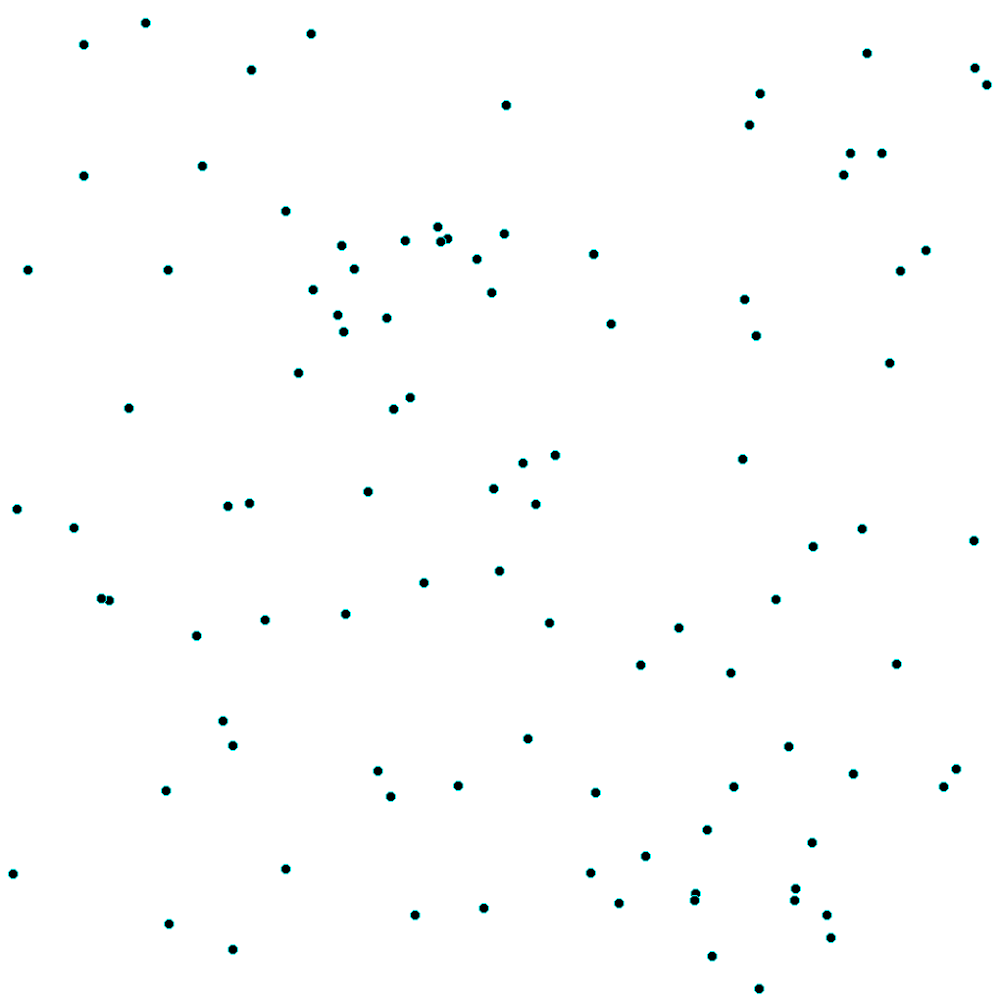
\includegraphics[width=0.60\textwidth]{chapters/experiments/img/uniform_example.png}
    \caption{Wizualizacja wygenerowanej instancji z miastami rozmieszczonymi równomiernie dla N=100}
    \label{fig:uniform_example}
\end{figure}

\subsection*{Miasta rozmieszczone w klikach}
Miasta umieszczane są blisko siebie w kilku grupach oddzielonych większymi odległościami.
Przykład wygenerowanej instancji został przedstawiony na rysunku \ref{fig:clique_example}.
\begin{figure}[h!]
    \centering
    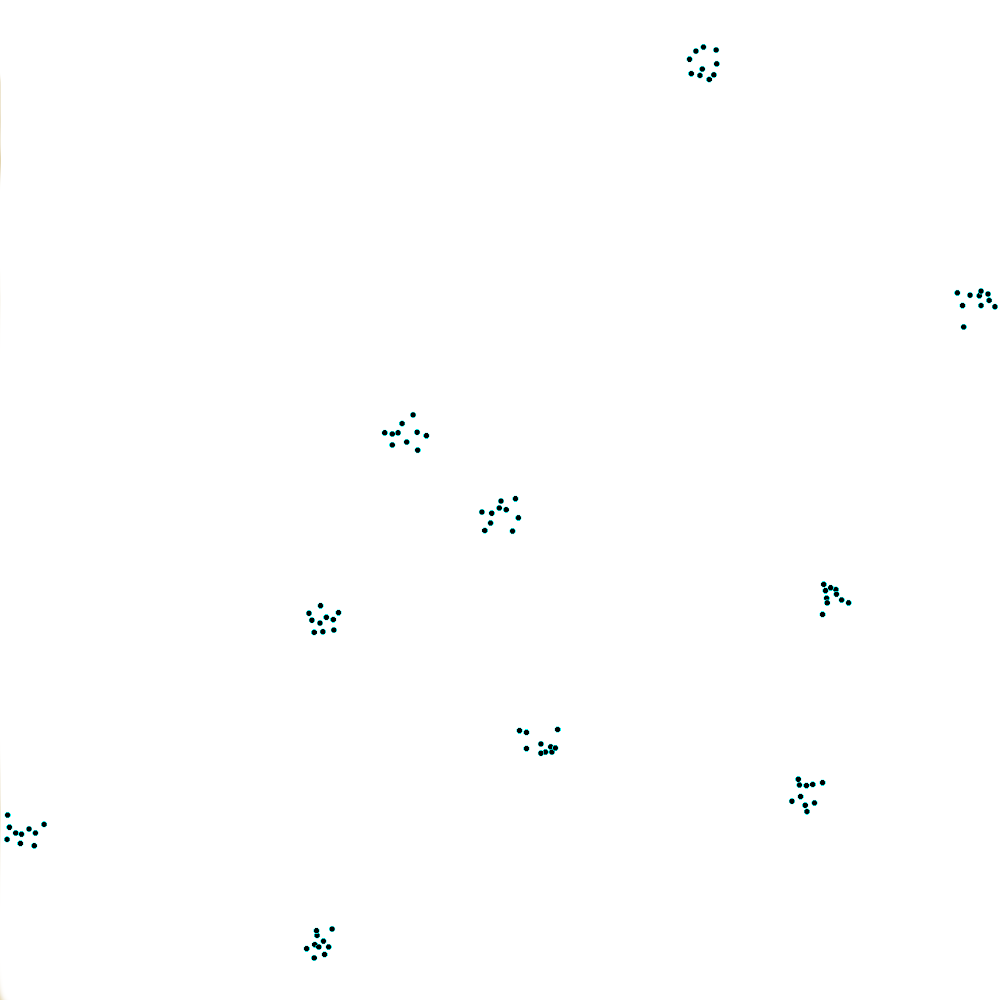
\includegraphics[width=0.60\textwidth]{chapters/experiments/img/clique_example.png}
    \caption{Wizualizacja wygenerowanej instancji z miastami rozmieszczonymi w kilkach dla N=100}
    \label{fig:clique_example}
\end{figure}

\subsection*{Miasta rozmieszczone na siatce}
Miasta umieszczane są na siatce, w stałej odległości od swoich sąsiadów.
Przykład wygenerowanej instancji został przedstawiony na rysunku \ref{fig:grid_example}.
\begin{figure}[h!]
    \centering
    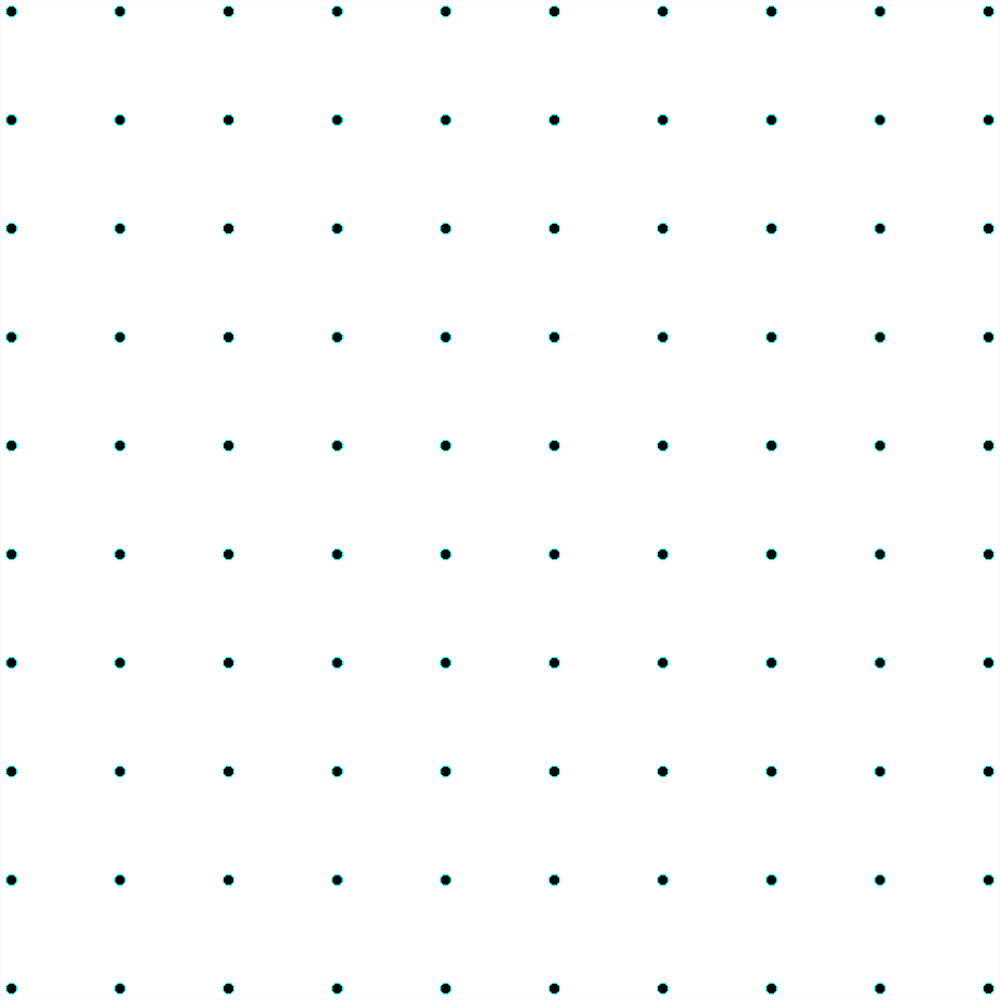
\includegraphics[width=0.60\textwidth]{chapters/experiments/img/grid_example.png}
    \caption{Wizualizacja wygenerowanej instancji z miastami rozmieszczonymi na siatce dla N=100}
    \label{fig:grid_example}
\end{figure}


Wygenerowano instancje testowe każdego z trzech typów instancji losowych o rozmiarach 7,8,9,10,11 oraz 20,50,100,200 i 500.
Uzyskano w ten sposób 30 instancji problemu.

Ze zbioru TSPLIB wybrano instancje o podobnych rozmiarach: \textbf{burma14}, \textbf{ulysses22}, \textbf{att58}, \textbf{berlin52}, \textbf{rat99},
\textbf{bier127}, \textbf{d198}, \textbf{a280}, \textbf{pa561}, \textbf{u574}.

\section{Experimental setup but po polsku}

\section{Wyniki}